\chapter{CaWaQS-Viz Features}
\label{chap-features}

\renewcommand{\headrulewidth}{0.3pt}
\fancyhead[LE]{\thepage} \fancyhead[RE]{\nouppercase{\textbf{\leftmark}}}
\fancyhead[RO]{\thepage} \fancyhead[LO]{\nouppercase{\textbf{\rightmark}}}
\fancyfoot[L,C,R]{}

\setlength{\parindent}{0.35cm}

\minitoc
\newpage
\

\newpage

% ================================================================
\alertwarning{All shapefile outputs generated by \cwv~are temporary. If they are not saved, they will no longer be accessible when the project is reopened.}

\section{\gui{Calibration Tools}: Calibration Tools}
\label{sec-calib-tools}

The \gui{Calibration Tools} dialog box (\cref{fig_DialogCalibrationTools})
provides access to the \cawaqs~model calibration tools. These features
are as follows:
\begin{itemize}
    \item a tool for modifying the parameterisation files of the various
        modelled compartments: \gui{Modify a parametrisation file} (\cref{sec-feat-modify-param})
        ;

    \item a tool for calculating model calibration performance criteria
        : \gui{Statistical Criteria} (\cref{sec-critstat}) ;

    \item a tool for calculating simulated run-off coefficients: \gui{Run-off coefficient calculation}
        (\cref{sec-runoff-coef}) ;

    \item a tool for visualizing simulated and observed time series: \gui{Compare sim/obs}
        (\cref{sec-com-simobs}).
\end{itemize}

\begin{figure}[H]
    \centering
    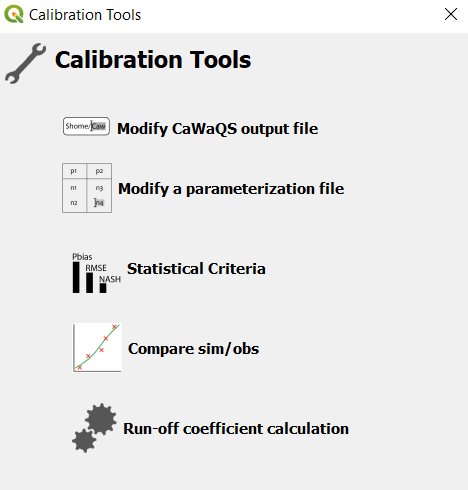
\includegraphics[width=0.65\linewidth]{
        2_application_user_guide/fig/DialogCalibrationTools.png
    }
    \caption{Calibration tools dialog box.}
    \label{fig_DialogCalibrationTools}
\end{figure}

\subsection{Modifying Parameterisation Files}
\label{sec-feat-modify-param}

Parameterisation files can be modified from the
\gui{Modifying a parametrization file} dialog box (\cref{fig-dialog_modif_param_file}).
The resolution will depend on the calibration file to be selected
from the drop-down menu. The table can be displayed by clicking on

\includegraphics[height=0.45cm]{2_application_user_guide/fig/show.png}
.\\

If the displayed attribute table does not contain the fields of the parameterisation file,
the resolution can be linked to its parameterisation file in the
\gui{Link resolution to its parameterisation file} dialog box, accessible by
clicking on
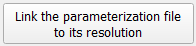
\includegraphics[height=0.55cm]{
    2_application_user_guide/fig/AccesDialogLinkParamResolution.png
}
. The use of this dialog box is described in \cref{sec-link_table}.

\begin{figure}[H]
    \centering
    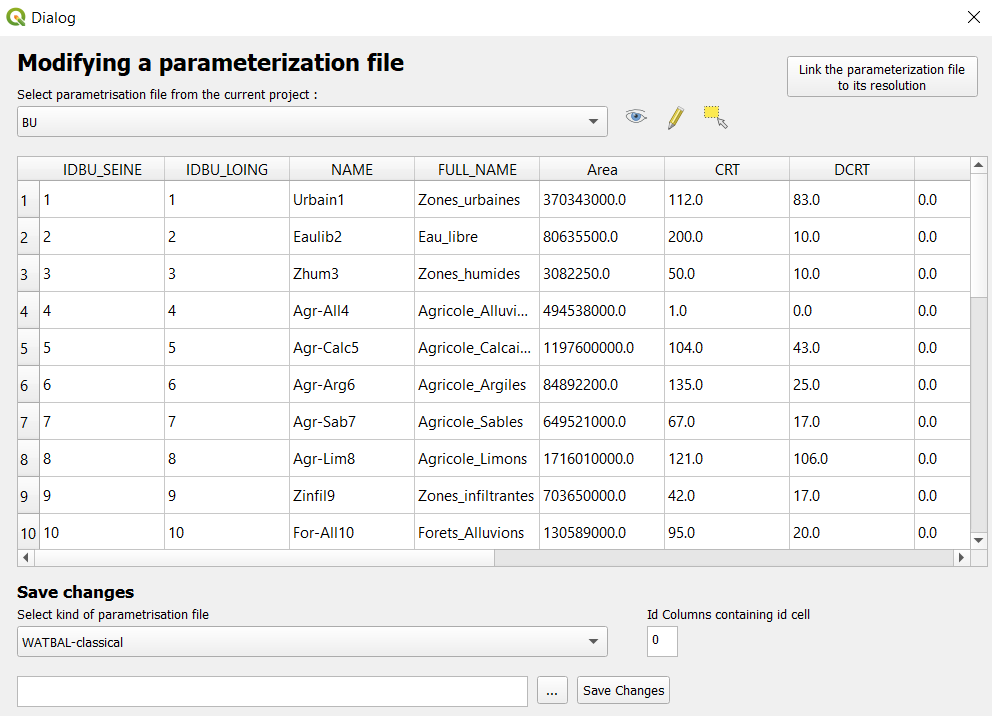
\includegraphics[width=1\linewidth]{
        2_application_user_guide/fig/DialogModifParamFile.png
    }
    \caption{Dialog box for modifying parameterisation files.}
    \label{fig-dialog_modif_param_file}
\end{figure}

Once the parameters have been modified in the displayed table, it can be
saved. The new file path can be specified by selecting

\includegraphics[height=0.45cm]{2_application_user_guide/fig/SelectPath.png}
. Specify the identifier of the column containing the cell identifier or name\footnote{ATTENTION: As a reminder, column identifiers start at \textbf{0}.}.

\subsection{Linking an Attribute Table to its Resolution}
\label{sec-link_table}

The parameters from the parameterisation file will be directly imported as
fields in the attribute table of the relevant resolution file. To create
this link, a parameterisation file type must be chosen (based on the compartment
and the type of parameterisation file), the \cawaqs~resolution, and the path
to this parameterisation file. Different types of parameterisation files
exist and are listed in table
\ref{tab-type_param_file}.

\begin{figure}
    \centering
    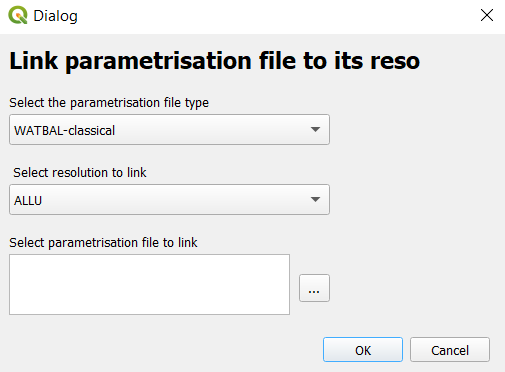
\includegraphics[width=0.7\linewidth]{
        2_application_user_guide/fig/DialogLinkTable.png
    }
    \caption{Dialog box for linking an attribute table to its resolution.}
    \label{fig:enter-label}
\end{figure}

\begin{table}[H]
    \centering
    \begin{tabular}{m{4cm}|m{4cm}|m{4cm}}
        \hline
        \textbf{Compartment} & \textbf{Parameterisation file type} & \textbf{Parameters listed in the table}             \\
        \hline
        \script{WATBAL}       & Classical                                   & CRT, DCRT, R, FN, CQR, CQRMAX, CQI, CQIMAX and RNAP       \\
        \hline
        \script{WATBAL}       & Infiltration Excess                         & CRT, DCRT, R, FN, CQR, CQRMAX, CQI, CQIMAX, RNAP and RINF \\
        \hline
        \script{AQ}           & Transmissivity                              & T                                                        \\
        \hline
        \script{AQ}           & Storage (storage coefficient)      & S                                                        \\
        \hline
        \script{AQ}           & Conductance                                 & C                                                        \\
        \hline
        % Add more data rows if necessary
    \end{tabular}
    \caption{Parameterisation files supported by \texttt{\cwv}.}
    \label{tab-type_param_file}
\end{table}

\subsection{\script{Statistical Criteria}: Calculation of Statistical Performance Criteria at Observation Points}
\label{sec-critstat}

The \gui{Statistical Criteria} dialog box (\cref{fig-dialogstatisticalcriteria})
returns a GIS layer following the geometries of the observation resolution
inherent to the analysed variable. Each field corresponds to a given statistical criterion. The selected statistical criteria are calculated over the period
specified in the \gui{Period for calculating statistical criteria} section.\\

\subsubsection{Statistical criteria calculated by the \gui{Statistical criteria} dialog box}

\textbf{\gui{Pbias} : Bias [$\%$]}
\begin{equation*}
PBIAS = \frac{\sum(\hat{y}_i -y_i)}{\sum y_i} . 100
\quad \quad
\begin{array}{rl}
      
      y_i & : \text{simulated variable at time $i$}\\
      O_i & : \text{observed variable at time $i$}\\
\end{array}  
\end{equation*}

\textbf{\gui{Average SIM/OBS}}
\begin{equation*}
    A = \overline{\hat{y}} - \overline{y}
    \quad\quad
    \begin{array}{cc}
         \overline{\hat{y}} :& \text{mean of simulated variables} \\
         \overline{y} : & \text{mean of observed variables}
    \end{array}
\end{equation*}

\textbf{\gui{Nash} : Nash-Sutcliffe Model Efficiency} \citep{nash1970}
\begin{equation*}
    NSE = 1 - \frac{\sum_{i=1}^n (y_i - \hat{y}_i)^2}{\sum_{i=1}^n (y_i - \overline{y})^2}
    \quad \quad 
    \begin{array}{ll}
         y_i :& \text{actual variable at time } i \\
        \hat{y}_i :& \text{predicted variable at time } i \\
    \end{array}
\end{equation*}

\textbf{\gui{RMSE} - Root Mean Squared Error} 
\begin{equation*}
RMSE = \sqrt{\frac{1}{n} \sum_{i=1}^{n} (y_i - \hat{y}_i)^2}
\quad \text{where} \quad
\begin{array}{ll}
    n :& \text{Total number of simulation days} \\
    y_i :& \text{actual variable at time } i \\
    \hat{y}_i :& \text{predicted variable at time } i \\
\end{array}
\end{equation*}

\textbf{\gui{KGE} - Kling-Gupta Efficiency} \citep{gupta2012}
\begin{equation}
    KGE = 1 - \sqrt{(r - 1)^2 + (\alpha - 1)^2 + (\beta - 1)^2} 
    \quad \quad
    \begin{array}{ll}
         r & : \text{Pearson correlation coefficient} \\ 
         & \text{between the simulated and observed} \\ 
         & \text{variable series} \\
        \alpha & : \text{ratio of simulated and observed standard deviations} \\
        \beta  & : \text{mean bias between simulated and observed series}
    \end{array}
\end{equation}




The following criteria are calculated automatically: $\overline{y}$, $\overline{\hat{y}}$, $\frac{\overline{\hat{y}}}{\overline{y}}$, $\sigma y$,  $\sigma \hat{y}$, $\frac{\sigma \hat{y}}{\sigma y}$.

\subsubsection{Output of the \gui{Statistical Criteria} dialog box}
\label{sec_stats_crits}

The dialog box generates statistical criteria: 
\begin{itemize}
    \item at observation points,  
    \item at the scale of the aquifer layer in the case of a simulation with an aquifer compartment;
    \item at the scale of the hydrosystem in the case of a simulation with an aquifer compartment.
\end{itemize}
\vspace{0.3cm}

\underline{\textbf{Statistical criteria calculated at observation points}}\\
The dialog box generates the statistical criteria table at observation points in \script{shapefile} and \script{text} format. The Shapefile is introduced directly into the current \script{QGIS} project, while the text file will be found in the \script{../PostProcessing/STATS\_CRITS} directory. 
The output criteria are contained in the fields of each measurement point under the names defined in table \ref{tab_statistical_criteria_crits_fields}.

\vspace{0.2cm}
\underline{\textbf{Statistical criteria calculated at the scale of aquifer units}}\\
In the case of a calculation of statistical criteria on the aquifer compartment, a \script{text} file is saved in the \gui{Post-Processing} directory under \script{../PostProcessing/STATS\_CRITS/AQ\_crits\_xxxx\_xxxx.txt}. This file lists the statistical criteria from table \ref{tab_statistical_criteria_crits_fields} defined at the scale of each aquifer unit. 

\vspace{0.2cm}
\underline{\textbf{Statistical criteria calculated at the hydrosystem scale}} \\
Statistical criteria are defined at the hydrosystem scale for the groundwater hydraulic head. These criteria are written in the file \script{../PostProcessing/STATS\_CRITS/AQ\_crits\_xxxx\_xxxx.txt}.\\


\begin{table}[H]
    \centering
    \renewcommand{\arraystretch}{1.2}
    \resizebox{\textwidth}{!}{
        \begin{tabular}{rl}
        \hline
        \textbf{Output table field name} &  \textbf{Statistical criterion} \\
        \hline
        \gui{NObs} & Number of observations over the selected period \\
        \gui{AObs} & Mean of observed variables \\
        \gui{ASIM} & Mean of simulated variables \\ 
        \gui{SUM\_RATIO} & Ratio of the sum of simulated variables to the sum of observed variables \\
        \gui{StdObs} & Standard deviation of observed variables \\ 
        \gui{StdSim} & Standard deviation of simulated variables \\
        \gui{STD\_RATION} & Ratio of standard deviations of observed and simulated variables \\
        \gui{PBAIS} & Bias [\%] \\
        \gui{AVERAGE\ SIM/OBS} & Mean ratio between simulated and observed variables \\
        \gui{KGE} & Kling-Gupta Efficiency \\
        \gui{NASH} & Nash-Sutcliffe Model Efficiency \\ 
        \gui{RMSE} & Root Mean Squared Error \\
        \hline
        \end{tabular}
    }
    \caption{Field names of output tables for each statistical criterion}
    \label{tab_statistical_criteria_crits_fields}
\end{table}


\begin{figure}[H]
    \centering
    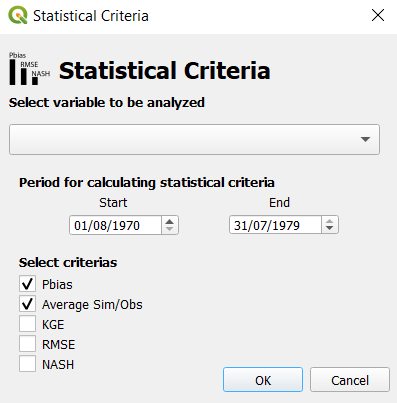
\includegraphics[width=0.5\linewidth]{
        2_application_user_guide/fig/DialogStatisticalCriteria.png
    }
    \caption{\gui{Statistical Criteria} dialog box.}
    \label{fig-dialogstatisticalcriteria}
\end{figure}


\subsection{\script{Run-off coefficient calculation}: Calculation of the Run-off Coefficient at Flow Measurement Stations}
\label{sec-runoff-coef}

This dialog box calculates the simulated and observed run-off coefficient at flow measurement stations.\\

\begin{figure}[H]
    \centering
    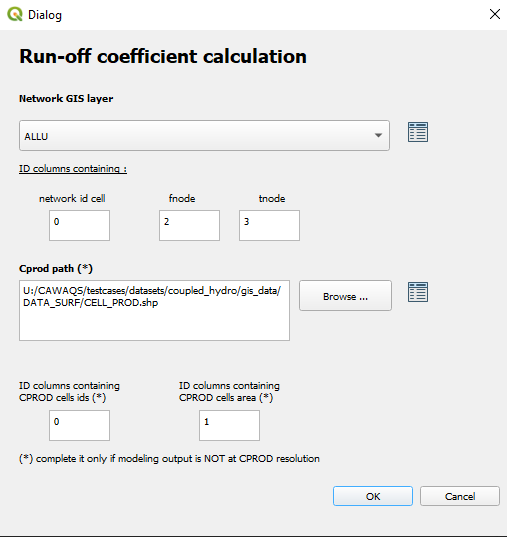
\includegraphics[width=0.5\linewidth]{
        2_application_user_guide/fig/DialogRunOffCalclulation.png
    }
    \caption{Dialog box for calculating the run-off coefficient.}
    \label{fig-DialogRunoffCoeff}
\end{figure}

This dialog takes as input the resolution of the surface hydrological scheme at the river reach scale and the \cawaqs~surface resolution of the production cells (unit catchments or \script{Cprod}). For the former, the column number containing the reach identifiers, \script{Fnode} and \script{Tnode} must be specified. For the latter, the identifiers of the fields containing the production cell identifier, and the cell area.\\

If the surface resolution defined in the \cwv~configuration is already that of production cells, it will not be necessary to fill in the lower part of the dialog box.

Two new resolutions (\textit{shapefiles}) will be returned by the dialog box and added to the current GIS project:
\begin{itemize}
    \item \gui{CATCH} which contains the catchments drained by each measurement
        station;

    \item \gui{CATCH\_SURF}, the product of the intersection between the surface resolution
        defined in the \cwv~configuration and \gui{CATCH}. Its attribute table
        contains several fields:
        \begin{itemize}
            \item[$-$] \gui{CATCH\_ID} and \gui{CATCH\_SURF}: the identifier of the
                catchment drained by the station and its area;

            \item[$-$] \gui{ID\_OBS}: the identifier of the measurement station;

            \item[$-$] \gui{SURF\_ID}: the area of the surface cell
                from the surface resolution defined in the \cwv~configuration;

            \item[$-$] \gui{SURF\_SURF}: its area;

            \item[$-$] \gui{INTER\_ID}: the identifier of the intersection cell;

            \item[$-$] \gui{INTER\_SURF}: the intersection area.
        \end{itemize}
\end{itemize}

These resolutions are saved in temporary format. It is left to the user
to save them for future reuse. If \cwv~recognises these
resolutions in the current QGIS project, they will be reused for calculating
run-off coefficients.\\

These coefficients can be found in the attribute table of the flow observation layer specified at the configuration step. Two new fields are then
added: \gui{QruissSim} and \gui{QruissObs} designating respectively the
run-off coefficient simulated by \cawaqs~and that observed at the measurement stations.

\section{\script{Compare sim/obs}: Comparison of Observed and Simulated Time Series}
\label{sec-com-simobs}

This calculation module enables comparison between simulations and observations through several types of output: 
\begin{itemize}
    \item by clicking on \gui{PDF printout}, a \script{pdf} file is generated. The simulated and observed time series are presented with the statistical criteria listed in table \ref{tab_statistical_criteria_crits_fields};
    \item by clicking on \gui{Interactiv graphics}, an \script{html} format reproduces the time series presentation format of the \script{pdf} interactively in the default browser;
    \item by clicking on \gui{Statistical criteria}, the \gui{Statistical Criteria} dialog box (\ref{sec-critstat}) opens. The parameters specified in the \gui{Compare Sim-Obs} dialog box (dates, compartment and observation unit of measurement) are transferred to the \gui{Statistical Criteria} dialog box. 
\end{itemize}

\begin{figure}[H]
    \centering
    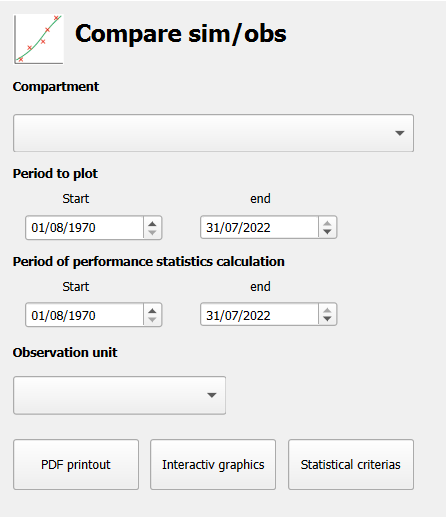
\includegraphics[width=0.45\linewidth]{
        2_application_user_guide/fig/DialogCompareSimObs.png
    }
    \caption{\gui{Compare sim/obs} dialog window.}
    \label{fig-dialogCompareSimObs}
\end{figure}

The compartment type (\script{AQ} = aquifer and \script{HYD} = hydrographic
network) is to be selected from the drop-down list located in the upper
part of the dialog box (\cref{fig-dialogCompareSimObs}). The time series printing periods and those for calculating statistical criteria must also be specified. The unit of flow observations, used for processing simulations of the \gui{HYD} compartment, must be specified in the \gui{Observation unit} drop-down menu. It is optional for processing the \gui{AQ} compartment.\\

An information message will be displayed in the QGIS interface at the end of this
task and will point to the post-processing directory. The
\script{.pdf} files resulting from analysis of the \script{HYD} compartment will be named
\gui{SIM\_OBS\_HYD.pdf} by default. Those from aquifer compartment analysis
will be named \gui{SIM\_OBS\_AQ.pdf}. Each page of this document corresponds to
a measurement station.

\section{\script{Spatial Map}: Spatial Mapping of Hydrological Variables}
\label{sec-spatial-map}

This tool spatialises the surface water balance in \script{.shp} format. The balance can be produced at an annual, monthly or daily frequency (to be specified in the \script{frequence} field). Temporal aggregation can be performed by mean, sum, maximum or minimum (to be specified in the \script{agregator} field).


\begin{figure}[H]
    \centering
    \begin{subfigure}
        [b]{0.48\linewidth}
        \centering
        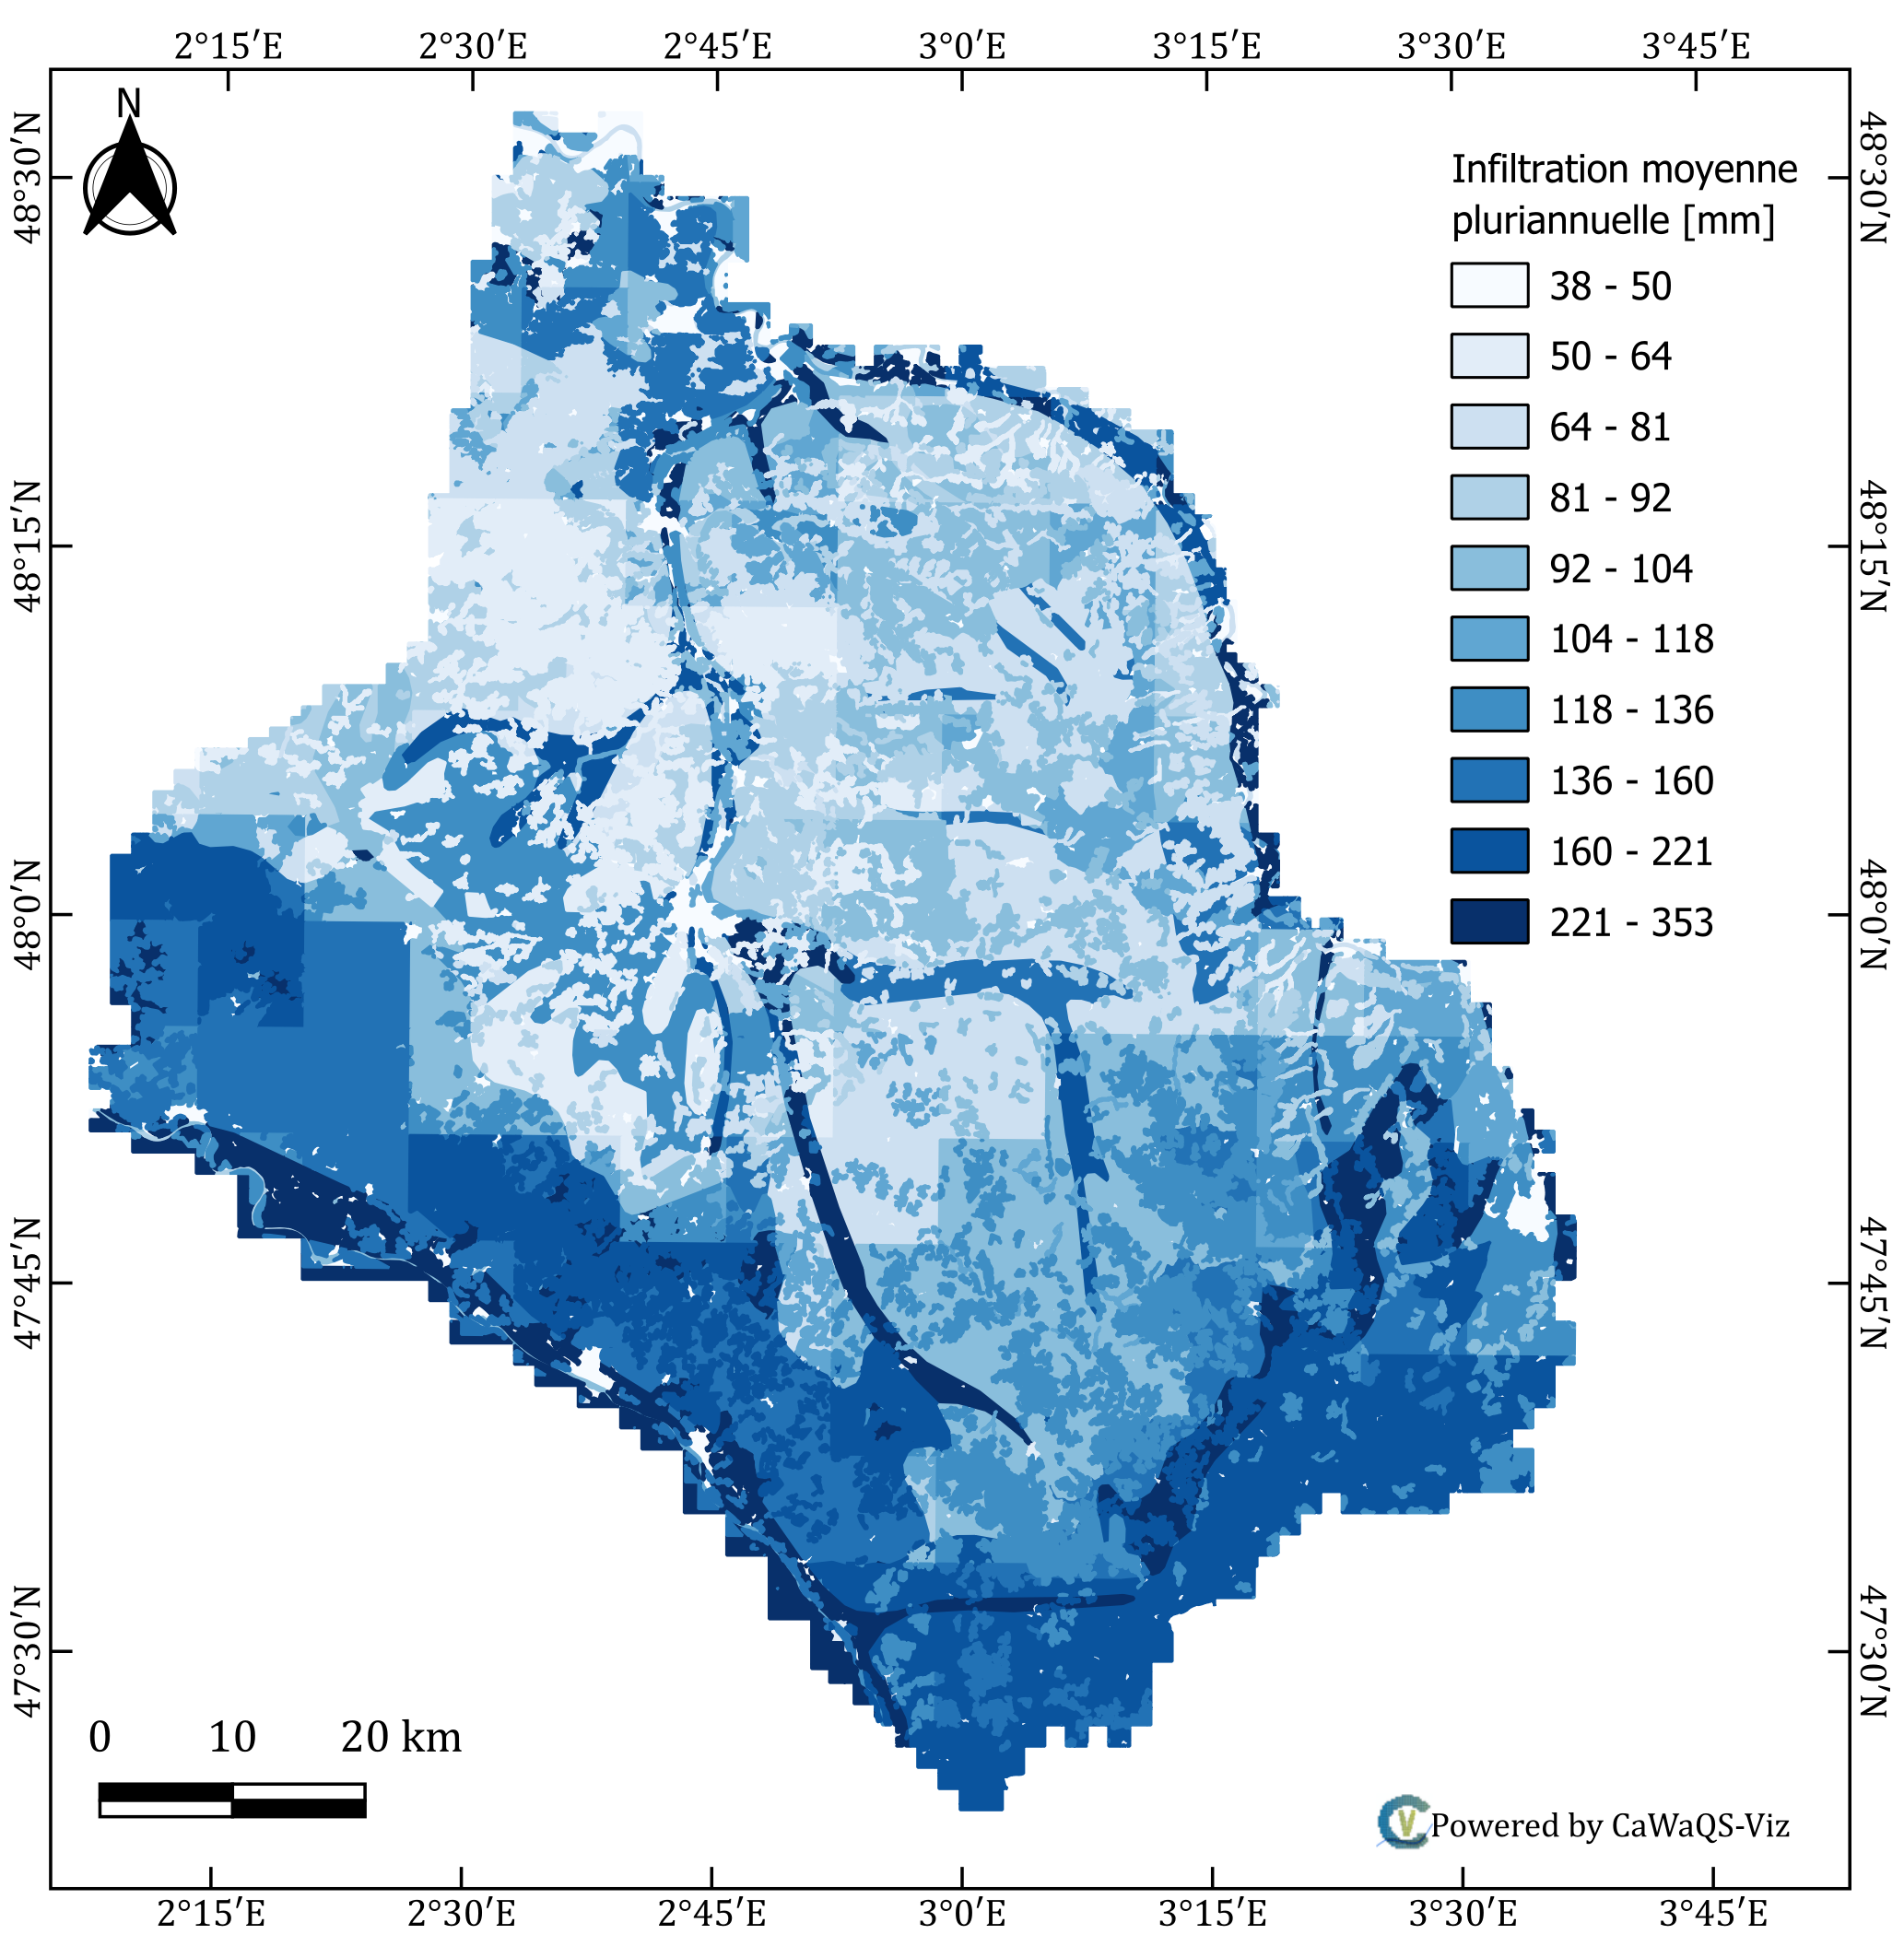
\includegraphics[width=\linewidth]{3_features/fig/OutputSpatialMap.png}
        \caption{}
        \label{fig-outSpatialMap-surf}
    \end{subfigure}
    \begin{subfigure}
        [b]{0.45\linewidth}
        \centering
        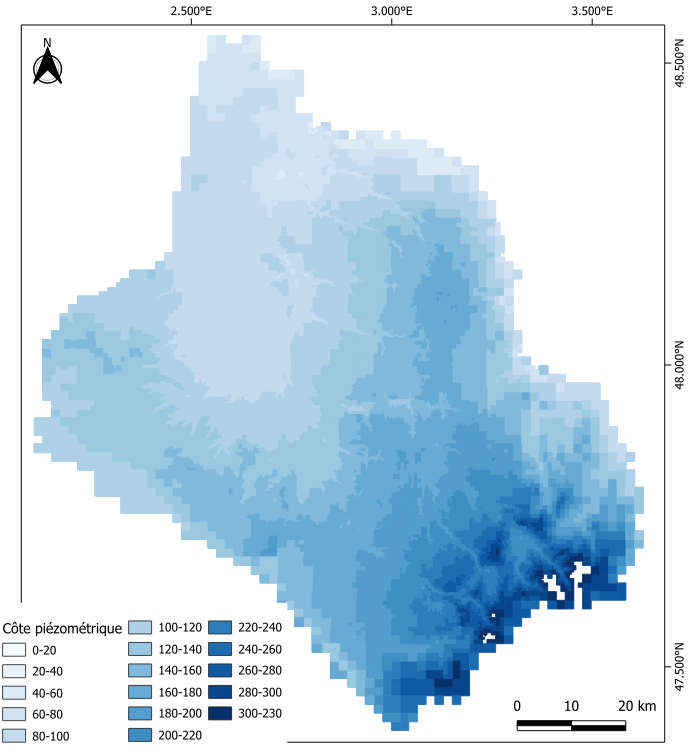
\includegraphics[width=\linewidth]{3_features/fig/Cote_piezo.png}
        \caption{}
        \label{fig-outSpatialMap-sout}
    \end{subfigure}
    \caption{Spatialisation of mean inter-annual infiltration flux [$mm$] (a)
    and piezometry [$mNGF$] (b) simulated at the scale of the Loing hydrosystem}
    \label{fig:two_figures}
\end{figure}

The values taken by the hydrological variable to be spatialised are contained in
the attribute table of the output \script{.shp} resolution. The table has as
columns the year identifiers for annual aggregation, the month identifiers for monthly aggregation and finally the date for daily time step output. A multi-year mean aggregation is also
possible by checking the \script{Pluriannual} box, thus establishing a
multi-year or multi-year monthly balance.

\begin{itemize}
    \item \script{WATBAL}: the precipitation, AET, runoff
        and infiltration variables (\ref{fig-outSpatialMap-surf});

    \item \script{AQ}: hydraulic heads (\ref{fig-outSpatialMap-sout}), viewable either on a given
        aquifer mesh layer, or on the outcropping aquifer cells
        (unique mesh, created by \cwv).\\
\end{itemize}

Variables from the \script{WATBAL} compartment are expressed in \mmj~or \mman~depending on
the chosen aggregation mode. Variables from the \script{AQ} compartment are expressed
in metres.

\section{\script{Budget Bar Plot}: Hydrological Budget Visualization}
\label{sec-bufget-barplot}

Simulated hydrological budgets can be visualized from this dialog box. They are constructed in accordance with the specified period. The \script{Frequences} field specifies the water balance calculation time step (multi-year, annual,
monthly or daily), while \script{agregator} specifies the temporal aggregator
(mean, sum, maximum, minimum). The water balance is spatially aggregated by
a mean of hydrological variables over all surface cells.

Upon execution of this dialog box, an \script{HTML} page opens in your
browser and displays an interactive hydrological budget chart. A static
image (cf. Fig. \ref{fig-budget-barplot}) of this same chart is
saved in the post-processing directory in a sub-folder \script{../BUDGET}
of the post-processing directory.

\begin{figure*}[htb]
    \centering
    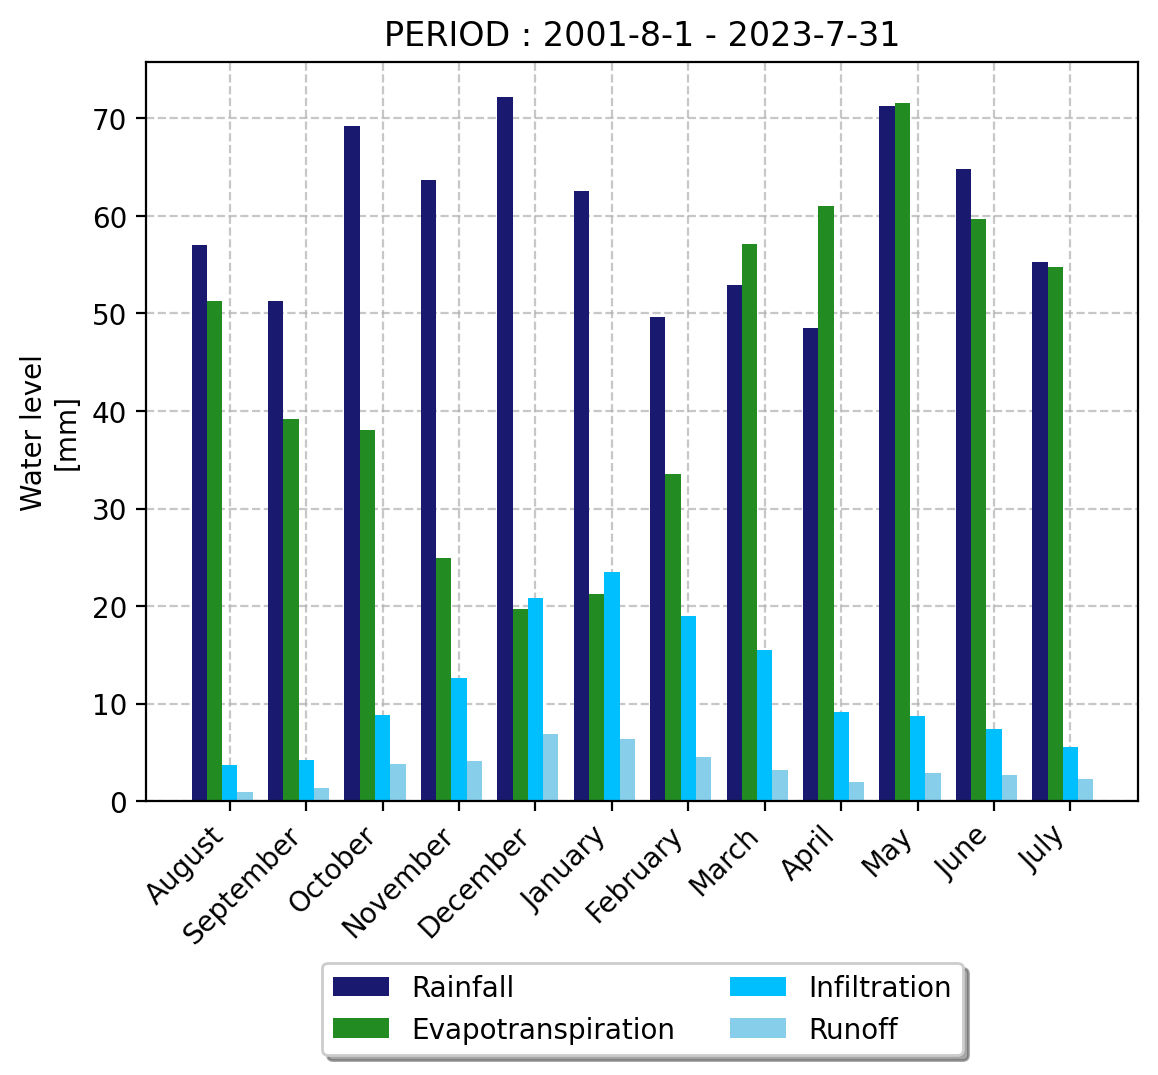
\includegraphics[width=0.55\linewidth]{
        3_features/fig/BUDGET_2001-8-12023-7-31Pluriannual_Sum.png
    }
    \caption{Example of a graphical output for the simulated multi-year monthly hydrological budget}
    \label{fig-budget-barplot}
\end{figure*}

\newpage
\section{\script{Hydological Regime}: Hydrological Regime Visualization}
\label{sec-regime-hydro}

The simulated hydrological regimes of the hydrosystem are constructed from the
\gui{Hydrological Regime} dialog box (cf. Figure
\ref{fig-dialogHydroRegime}). Hydrological regimes are calculated over the
period specified in the \gui{Start} and \gui{end} input fields. The variable
to be analysed is to be specified in the \gui{Hydrological variable to plot} drop-down menu. The output type is chosen by the user by checking the \gui{static plots (PNG)} box for graphical outputs as individual images for each measurement point, \gui{static plots (PDF)} for a PDF output compiling the hydrological regimes of all measurement points, and finally \gui{interractives plots} for an output in the default browser in the form of interactive charts (\ref{fig-output-regime-hydrologique}). A dialog box alerts the user when the calculation module has finished executing.\\

\begin{figure}[h]
    \centering
    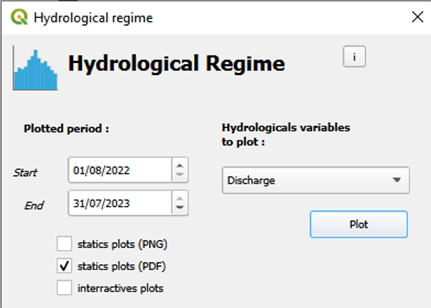
\includegraphics[width=0.5\linewidth]{
        3_features/fig/DialogHydrologicalREgime.png
    }
    \caption{\gui{Hydrological Regime} dialog box for calculating multi-year monthly hydrological regimes.}
    \label{fig-dialogHydroRegime}
\end{figure}


\begin{figure*}[htb]
    \centering
    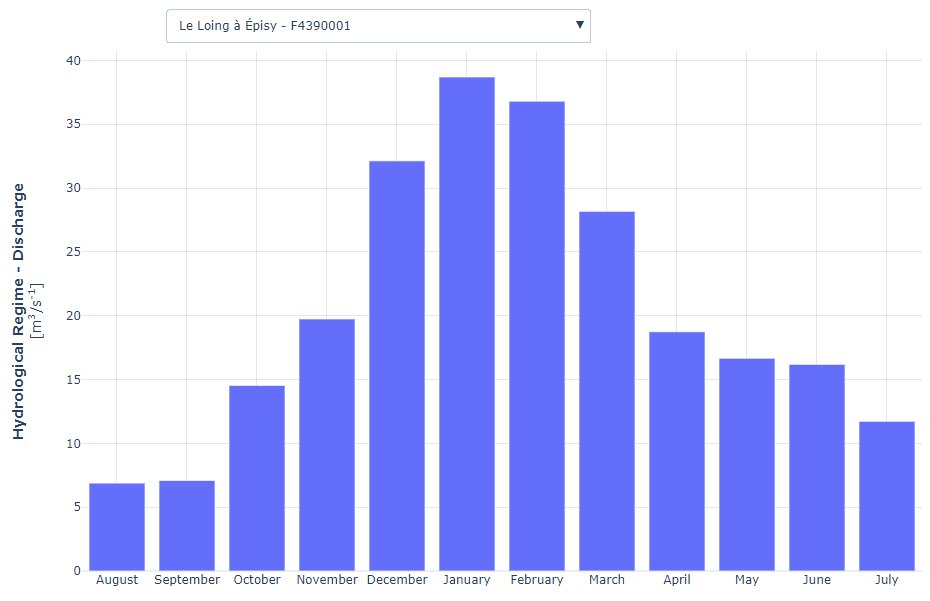
\includegraphics[width=0.5\linewidth]{
        3_features/fig/Output_regime_hydrologique.png
    }
    \caption{Example of a graphical output for the simulated multi-year monthly hydrological regime}
    \label{fig-output-regime-hydrologique}
\end{figure*}

\newpage
\section{\script{Extract Data from a sub area}: Extraction of Results in a Polygon}
\label{sec-extract-area}

The \gui{Extract Data from a Sub Area} dialog box allows extracting simulation results over a defined zone. This zone can be specified either as a polygon from a QGSVectorLayer loaded in the project, or as a shapefile imported from a directory.

Results are saved as CSV files (analyses) and NumPy files containing the data from the extracted zone. These files allow rerunning analyses from the created configuration.

\subsection*{Extraction variables}
From the dialog box, the following variables can be chosen for extraction:
\begin{itemize}
    \item Name of the new extraction file (also used as the name of the folder created in \texttt{PostProcessing/DATA\_EXTRACTED/})
    \item Extraction polygon: either a shapefile (to be tested) or a QGSVectorLayer present in the project
    \item Extraction period
    \item Extraction resolution for the WATBAL module (to be confirmed if necessary)
\end{itemize}

The outputs depend on the boxes checked in the right-hand column.

\subsection*{Outputs -- Hydrological balance (WATBAL)}
\gui{Rainfall} \gui{Real EvapoTranspiration (ET)} \gui{Infiltration} \gui{Runoff} \gui{Potential EvapoTranspiration (ET)}

These options provide the results of the hydrological balance (WATBAL). Data are saved in a CSV file in aggregated form over the entire simulation period, with one value per cell.

\subsection*{Outputs -- Hydrological regime (HYD)}
\gui{Surface flow}

\begin{itemize}
    \item All reaches in contact with the polygon boundary are defined as extraction points.
    \item The CSV file contains daily flow and water level data for each point located on the polygon boundary.
    \item The sign convention for flow is: positive for inflow, negative for outflow.
    \item NumPy files are also generated, allowing further analysis of these data.
\end{itemize}

\subsection*{Outputs -- Aquifer}
\gui{Subsurface flow}

\begin{itemize}
    \item For each aquifer layer, the polygon boundaries are defined with the resolution specific to that layer.
    \item A CSV file is generated for each layer.
    \item Fluxes are provided at a daily scale for each face located at the aquifer boundary.
    \item Faces are named according to the convention: \texttt{nCell(ID\_ABS)\_direction\_unit}, for example: \texttt{3323\_west\_m3d}.
\end{itemize}

\subsection*{Output Organisation}

For each extraction, result files and layers are produced.

Files are saved in the output directory defined in the main analysis parameters:
\texttt{PostProcessing/DATA\_EXTRACTED/<Extraction\_Name>}

Contents:
\begin{itemize}
    \item \textbf{CONFIG/}: configuration files for rerunning simulations
    \item \textbf{OUTPUT/}: CSV files containing the results
    \item \textbf{TEMP/}: NumPy files used to rerun analyses
\end{itemize}
